\section{Dossier de conception}

\subsection{Diagramme de classes}
\label{sec:diagramme-de-classes}

\begin{figure}[h!]
  \centerline{
  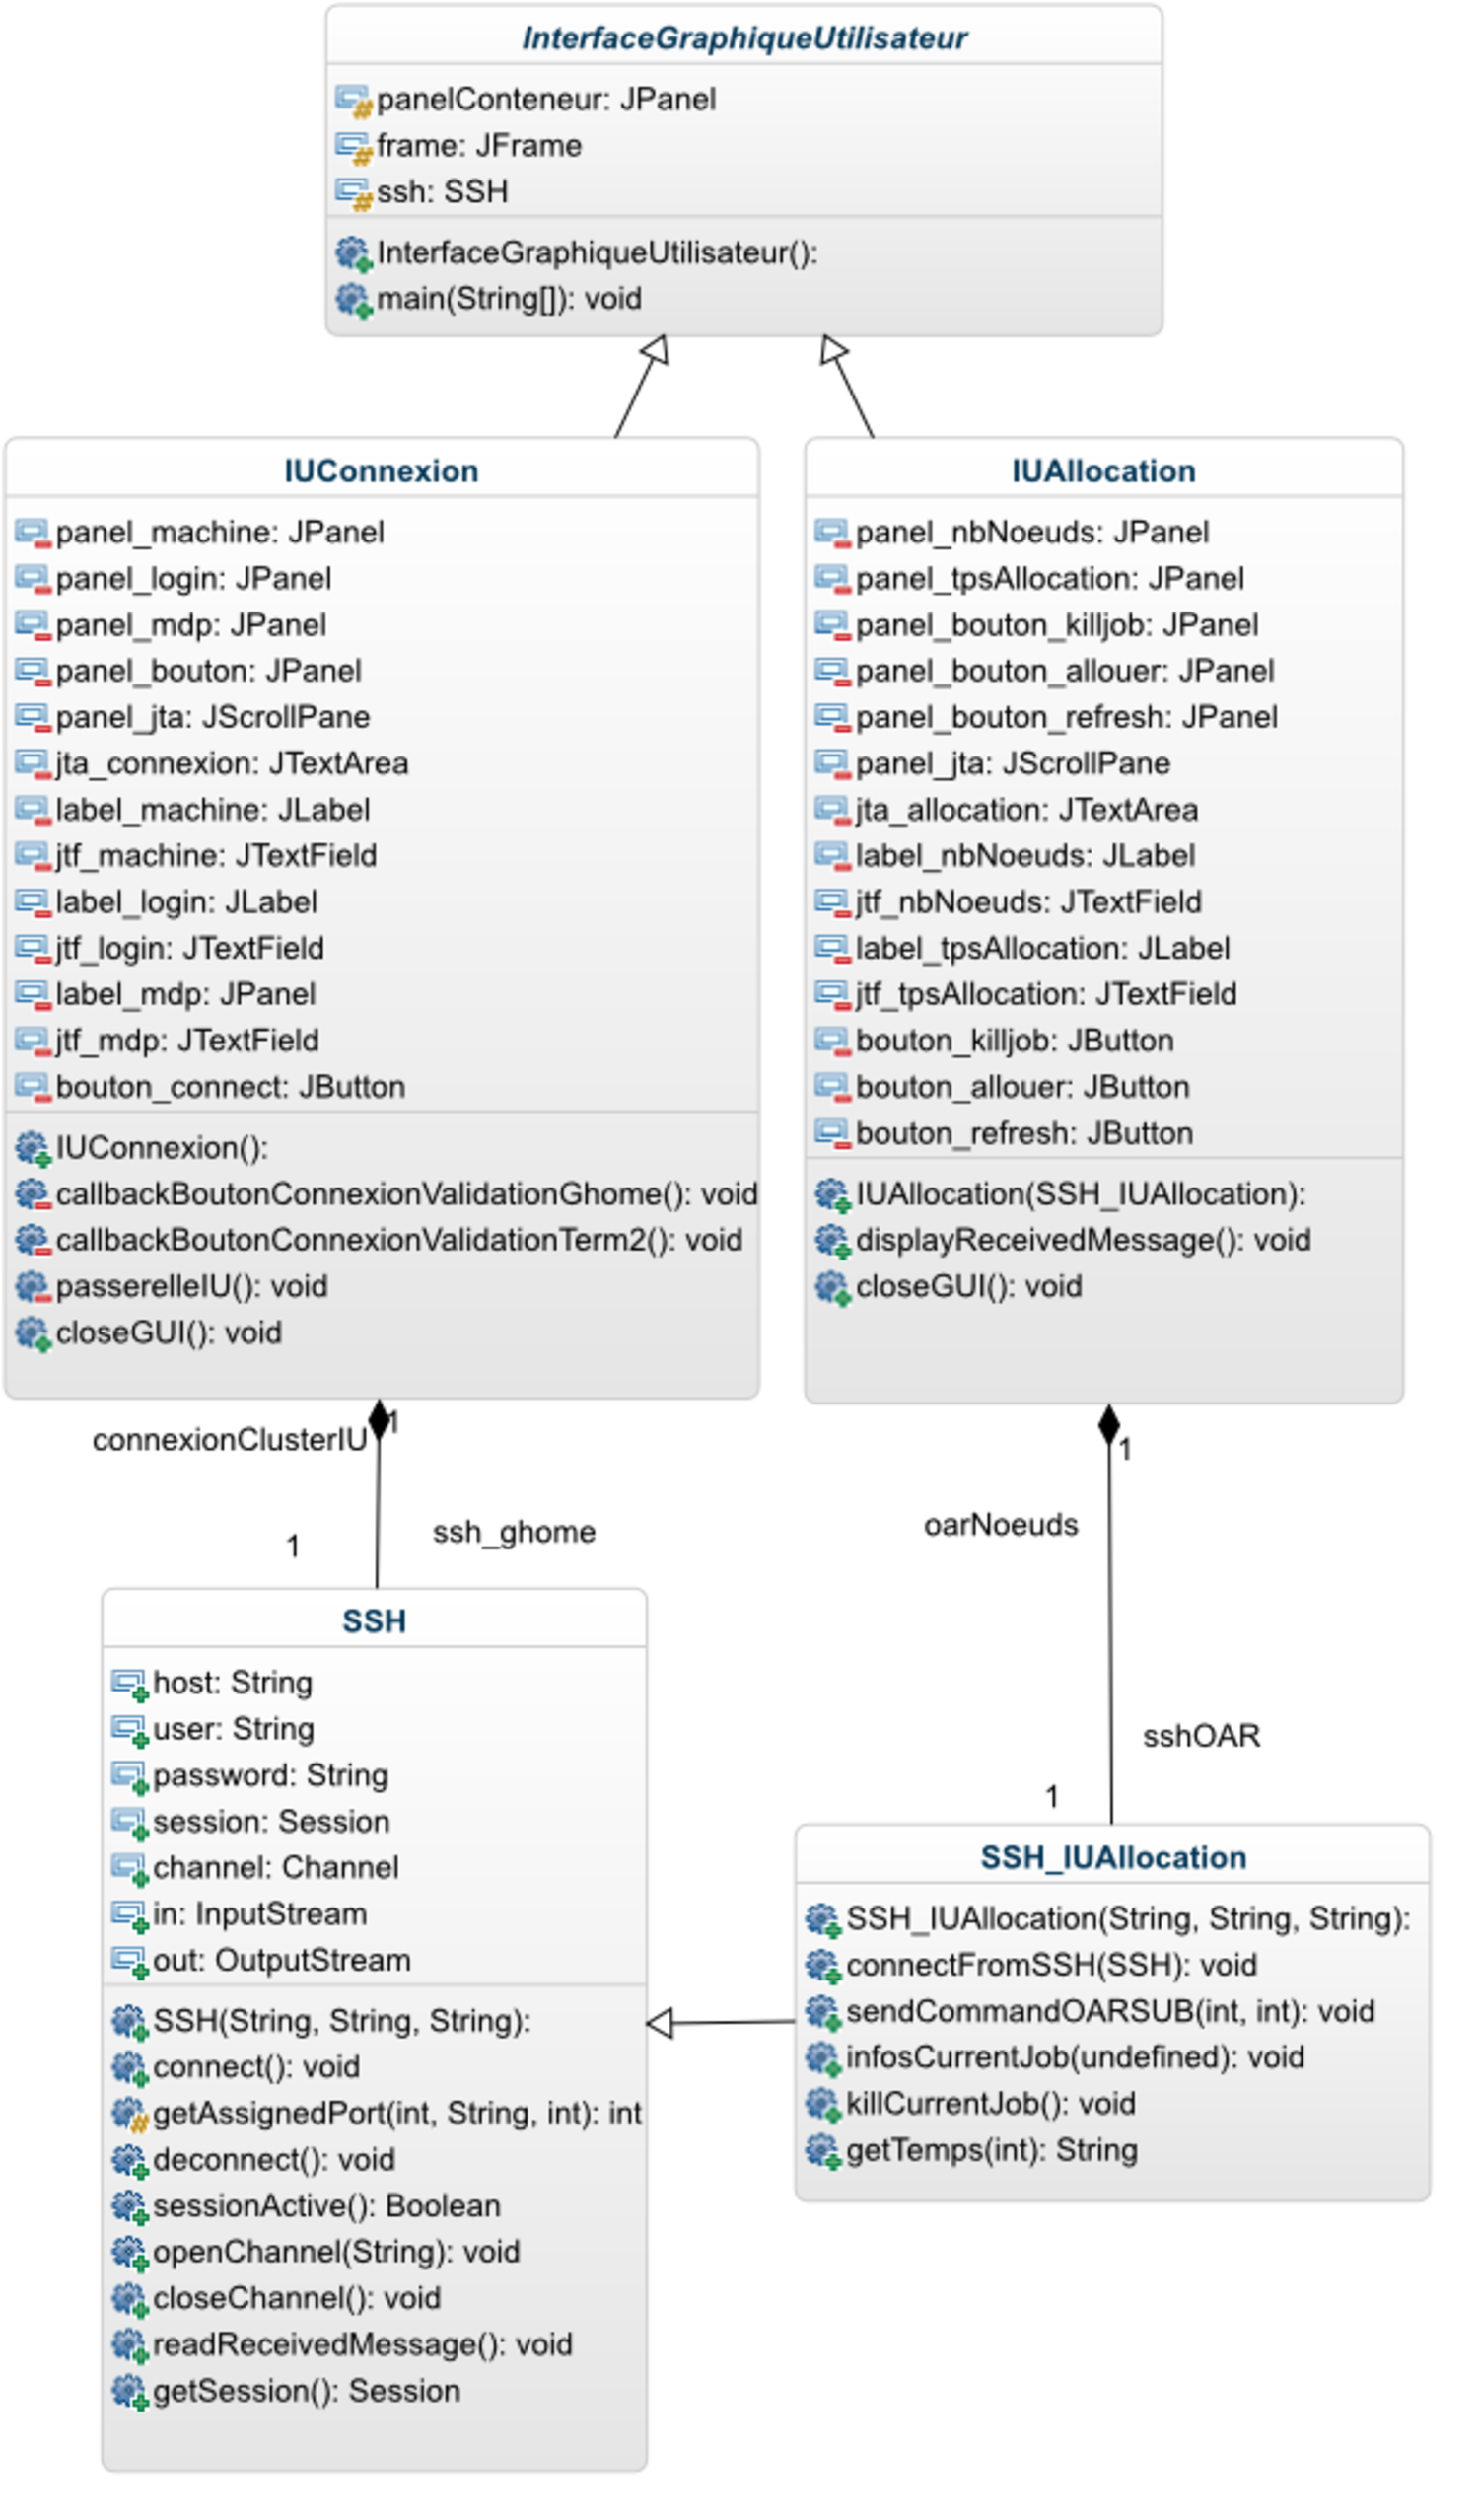
\includegraphics[width=18cm]{images/diagramme_classes.png}}
  \caption{Diagramme des classes}
  \label{fig:diag_classes}
\end{figure}

\subsection{Diagramme de séquence}
\label{sec:diagr-de-sequ}

\begin{figure}[h!]
  \centering
  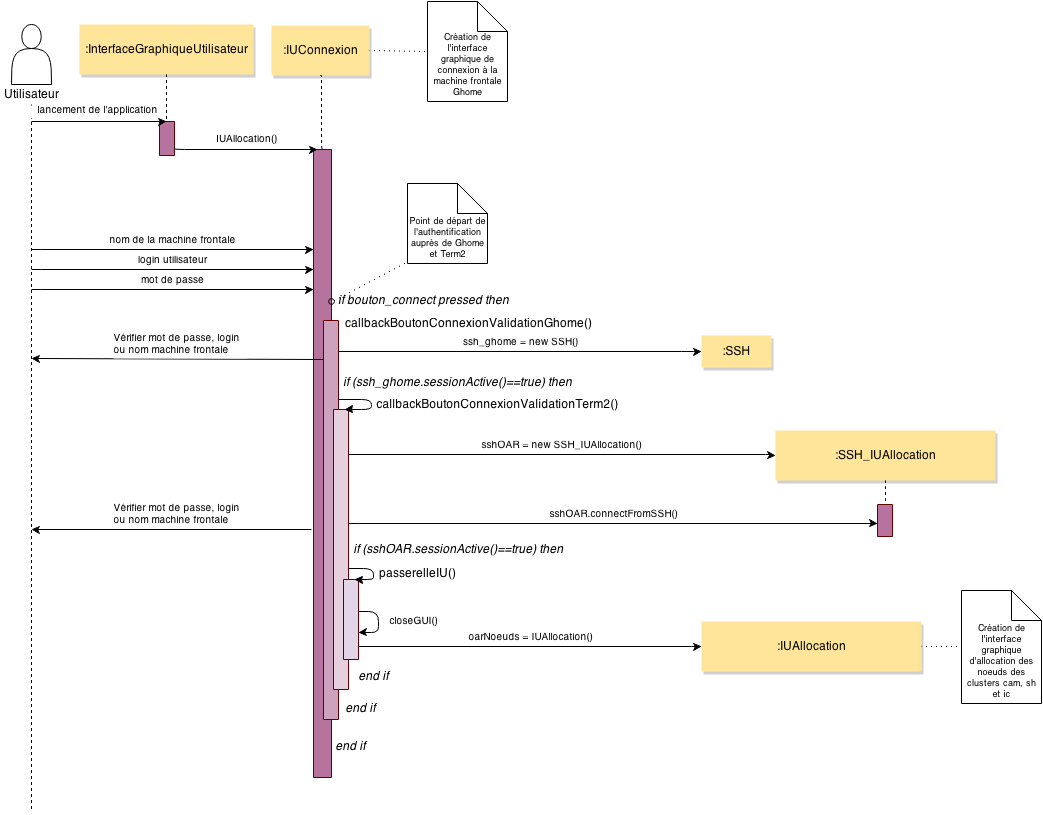
\includegraphics[width=16cm]{images/diagramme_sequence.png}
  \caption{Diagramme de séquence}
  \label{fig:diag_seq}
\end{figure}

\par La figure \ref{fig:diag_seq} donne le diagramme de séquence du scénario «Créer un job».  Tout d’abord, au lancement de l’application par l’utilisateur, l’IU de connexion s’affiche. L’utilisateur est en mesure de renseigner la machine sur laquelle il souhaite se logger, son nom d’utilisateur ainsi que son mot de passe. Lorsque les champs ont été convenablement remplis, l’appui sur le bouton de connexion lance le processus d’identification auprès des serveurs.
\par Une première session ssh est créée dans le serveur GHOME à partir de laquelle, sous condition qu’elle soit active, est créée une deuxième session ssh dans le serveur \texttt{TERM2}. S’il est impossible d’ouvrir une des deux sessions, alors un message d’erreur est renvoyé à l’utilisateur lui demandant de remplir à nouveau les champs. Dans le cas contraire, l’IU de connexion laisse sa place à l’IU d’allocation et le channel de type shell est créé afin d’envoyer les commandes au serveur.
\par L’utilisateur est désormais en mesure de remplir les champs «Nombre de nœuds» et «Temps d’allocation (en min)». L’appui sur le bouton allouer permet d’exécuter la commande ssh. Pour ce faire, plusieurs étapes sont nécessaires. Tout d’abord, les données rentrées par l’utilisateur doivent être traitées et mises sous forme d’une commande shell. La méthode \texttt{sendCommandOARSUB(nbNoeuds, tpsAllocation)} réalise cela en faisant appel à la méthode \texttt{getTemps(int)} afin de mettre sous forme xx:xx:xx heure:minutes:secondes) le temps d’allocation donné en minutes. La commande shell est créée et envoyée via le channel préalablement ouvert.
\par Une fois la commande shell envoyée, la méthode \texttt{readReceivedMessage()} se charge de rediriger vers l’utilisateur, à travers la \texttt{JTextArea} intégrée dans l’IU d’allocation, les données  renvoyées par le serveur. Ces données comprennent, conformément au cahier des charges la liste de nœuds alloués ainsi que les données décrivant l’état de création du job. 
\par Le rafraîchissement de la lecture des données en input du channel, donc provenant du serveur, est assuré par un objet de type Timer ayant pour but toutes les demi secondes de prendre la main afin de tester la présence de données en input. Les données retournées par le serveur semblent donc provenir en continu, sans que l'écoute ne monopolise le thread EDT.
\par Deux cas de figure se présentent à nous désormais concernant le scénario «Tuer le job». Soit le temps d’allocation est écoulé et dans ce cas le job est tué automatiquement par le serveur. Dans ce cas de figure le serveur se charge de reprendre les nœuds qu’il avait alloués. Donc aucune méthode java n’est nécessaire. 
\par Soit l’utilisateur a réalisé une mauvaise manipulation et n’a pas alloué le bon nombre de nœuds ou les a alloués pour une durée trop courte/trop longue (cf. scénario «Tuer le job»). Ici, l’utilisateur aura la possibilité de tuer le job afin d’en créer un nouveau à l’aide du bouton tuer qui appel la méthode \texttt{killCurrentJob()}. Cette méthode va tout simplement construire et envoyer la commande shell permettant de tuer le job courant en allant chercher au sein des variables d’environnement générées par OAR lors de la création du job son identifiant. Ceci évitera par exemple de tuer le job de quelqu’un d’autre.

%%% Local Variables: 
%%% mode: latex
%%% TeX-master: "CompteRendu"
%%% End: 
